\documentclass[conference]{IEEEtran}
\usepackage[T1]{fontenc}
\usepackage{amsmath}
\usepackage{graphicx}
\usepackage{booktabs}
\usepackage{algpseudocode}
\usepackage{cite}

\newcommand{\wmrf}{WMRF-LG}
\newcommand{\wdrf}{Weighted DRF-inspired}

\title{Fair Resource Allocation for Mixed Batch, Interactive and AI-Inference Workloads in Cloud Computing}
\author{\IEEEauthorblockN{Akshith Veerisetty, Sajja Venkata Naveen, Pitti Aswarth Narayana}
\IEEEauthorblockA{IIIT Sri City}}

\begin{document}
\maketitle

\begin{abstract}
Cloud schedulers allocate processor and memory capacity across workloads with different demands and service-level agreements (SLAs). Workload-Aware Weighted Multi-Resource Fairness with Latency Guard (WMRF-LG) combines rolling dominant-resource reservation-time accounting, bounded latency urgency, and task ageing with work-conserving admission for Batch, Interactive, and artificial intelligence (AI) inference workloads. CloudSim Plus experiments compared WMRF-LG, first-come, first-served (FCFS), Strict Priority, and a weighted Dominant Resource Fairness-inspired heuristic. Four workload mixes, two configurations, and 20 matched seeds yielded 640 comparative runs, 640 ablation runs, and 153,600 task completions. The evaluation separates SLA misses among intrinsically feasible tasks from tasks whose ideal CPU service time already exceeds the response-time target. Under Balanced original stress, WMRF-LG reduced mean Interactive response by 67.27 seconds relative to FCFS. Under Inference-heavy original stress, it reduced mean per-run maximum Batch queue wait by 153.12 seconds relative to Strict Priority while increasing mean inference response by 70.33 seconds. Strict Priority led on mean Interactive response in all eight strata, and FCFS led on mean throughput in seven. Ablation showed workload-dependent latency effects and no consistent reduction in Batch waiting from ageing. The choice of policy depends on workload mix and performance objective.
\end{abstract}

\begin{IEEEkeywords}
Cloud computing, resource allocation, multi-resource scheduling, dominant resource fairness, latency-aware scheduling, mixed workloads.
\end{IEEEkeywords}

\section{Introduction}
Cloud clusters share finite processor and memory capacity among services with different performance objectives. Co-locating user-facing and best-effort work can use otherwise idle capacity, but it also creates contention and exposes latency-sensitive services to delays \cite{verma2015borg,lo2015heracles}. In this study, Batch represents long-running best-effort work, Interactive represents short user-facing requests with a response-time target, and artificial intelligence (AI) inference represents compute- and memory-intensive requests with a separate target. A single fixed priority can repeatedly defer Batch, while first-come, first-served (FCFS) gives older Batch tasks precedence even when newer requests have deadlines. A fair-share policy based on relative resource use can account for CPU and random-access memory (RAM) contention across classes. Current resource shares alone provide no direct signal about either deadline slack or elapsed queue wait.

The research question is how to allocate CPU- and RAM-constrained cloud resources among Batch, Interactive, and AI-inference workloads while balancing latency, throughput, fairness, and workload protection. The project contributes an arrival-driven dispatcher with atomic CPU/RAM admission and a matched-trace comparison of \wmrf{} with three baselines. \wmrf{} uses rolling dominant-resource reservation-time accounting to track class shares. A two-factor ablation isolates the effects of bounded urgency and ageing.

\section{Related Work}
\subsection{Cluster management and multi-resource fairness}
Borg uses admission control, packing, reclamation, and isolation to share clusters between long-lived services and batch jobs. Verma \emph{et al.} analyze production clusters and simulate placement from production checkpoints to quantify the capacity cost of separating production and non-production work \cite{verma2015borg}. Here the virtual topology and placement rule stay fixed across dispatch policies.

Dominant Resource Fairness (DRF) extends max-min fairness to heterogeneous demands through normalized dominant shares. Ghodsi \emph{et al.} also analyze weighted shares and evaluate DRF in Mesos \cite{ghodsi2011drf}. Choosy extends max-min sharing to placement-constrained jobs and evaluates online allocation in experiments and simulation \cite{ghodsi2013choosy}. To reduce the cost of computing fair allocations at scale, Soroush uses single-shot optimization and generalized water filling. Namyar \emph{et al.} evaluate it on network flows and generated heterogeneous GPU training jobs, and deploy it for Azure traffic engineering \cite{namyar2024soroush}. These works concern fairness of allocations. \wmrf{} uses class entitlements to rank discrete admissions from recent CPU/RAM reservations.

\subsection{Co-location, latency and inference}
Heracles uses feedback control of CPU, cache, memory bandwidth, and other shared resources to limit interference between latency-critical services and best-effort jobs, evaluated with production workloads \cite{lo2015heracles}. Sinan addresses cascading latency violations in interactive cloud microservices by predicting tail latency and adjusting per-tier CPU allocations. Zhang \emph{et al.} benchmark it on end-to-end hotel reservation and social network applications under varying loads \cite{zhang2021sinan}. In this study, a bounded urgency term changes task order under fixed VM capacities.

Clockwork uses predictable execution and explicit model-placement decisions to schedule deep neural network inference, evaluated on graphics processing units (GPUs) with real models and request traces \cite{gujarati2020clockwork}. Llumnix addresses variable large language model inference demands by migrating live requests and their state across GPU replicas. Sun \emph{et al.} assess tail latency and priority isolation with a serving prototype and trace-based workloads \cite{sun2024llumnix}. The present simulator represents inference requests as CPU/RAM-constrained Cloudlets.

The literature reviewed here motivates an empirical question about how rolling weighted dominant-resource reservation-time accounting, bounded latency urgency, task ageing, work-conserving borrowing, and atomic CPU/RAM admission interact when Batch, Interactive, and AI-inference tasks share one dispatch framework. The comparison and ablation address this question for the workloads and assumptions defined below.

\section{Methodology}
\subsection{System model}
The discrete-event model uses CloudSim Plus \cite{silva2017cloudsim}. The datacenter has three physical hosts, each with four processing elements (PEs) at 1,000 million instructions per second (MIPS) per PE, 16,384 MB RAM, 10,000 Mb/s bandwidth and 1,000,000 MB storage. Six virtual machines (VMs) each request two PEs at 1,000 MIPS per PE, 4,096 MB RAM, 1,000 Mb/s bandwidth and 20,000 MB storage. The hosts provide 12 PEs and 49,152 MB RAM in total. The VMs request 12 PEs and 24,576 MB RAM in total. The dispatch policies operate on capacity available within the VMs. Both host VM scheduling and VM Cloudlet execution are space-shared. Each admitted Cloudlet uses its assigned PEs at full modeled CPU demand and holds its PE and RAM reservations until release.

\subsection{Workload model}
Table~\ref{tab:profiles} gives the original stress profiles. Length is measured in millions of instructions (MI) per PE, so a task requesting multiple PEs executes its declared MI on each of those PEs. Batch is best effort with no service-level agreement (SLA) for response time. Interactive has a 5 s target, and AI inference has a 10 s target. The simulation uses CPU/RAM-intensive inference-like Cloudlets. Model execution and GPU inference are outside its scope.

\begin{table}[t]
\caption{Original stress workload profiles and class entitlements}
\label{tab:profiles}
\centering
\begin{tabular}{@{}lrrrc@{}}
\toprule
Class & MI per PE & PEs & RAM (MB) & Weight\\
\midrule
Batch & 30,000--120,000 & 1--2 & 1,024--2,048 & 0.30\\
Interactive & 2,000--10,000 & 1 & 256--1,024 & 0.35\\
AI inference & 10,000--50,000 & 1--2 & 1,536--3,072 & 0.35\\
\bottomrule
\end{tabular}
\end{table}

Each trace contains 120 tasks in one of four mixes (Table~\ref{tab:mixes}). A seeded Java generator uses separate random streams for arrivals, class shuffling, and resource draws. It shuffles the class labels and accumulates exponential inter-arrival times at rate $0.5\,\mathrm{s}^{-1}$. It samples length, PE count and RAM uniformly over their inclusive integer ranges. The 600 s arrival horizon is a validation bound. A trace exceeding the bound is rejected as a whole.

\begin{table}[t]
\caption{Fixed class counts per 120-task trace}
\label{tab:mixes}
\centering
\begin{tabular}{@{}lrrr@{}}
\toprule
Scenario & Batch & Interactive & AI inference\\
\midrule
Balanced & 48 & 42 & 30\\
Batch-heavy & 72 & 24 & 24\\
Interactive-heavy & 24 & 72 & 24\\
Inference-heavy & 24 & 24 & 72\\
\bottomrule
\end{tabular}
\end{table}

For a task $j$ with length $\ell_j$ in MI per PE, the ideal service bound $b_j$ is $\ell_j$ divided by the fastest MIPS per PE of a VM whose configured capacity can accommodate its PE and RAM requests. A task with target $\tau_j$ is intrinsically feasible when $b_j\leq\tau_j$ and intrinsically infeasible otherwise. Equality permits zero ideal queueing slack. The analysis evaluates the approved original stress workload and the separately named, unapproved demonstration candidate \texttt{service-bound-demo-unapproved}. The candidate preserves arrivals, class labels, PE and RAM draws, targets and Batch lengths. A separate random stream initialized with the trace seed resamples Interactive lengths in $[2{,}000,5{,}000]$ MI per PE and sets inference lengths to 10,000 MI per PE. These changes make all candidate SLA tasks intrinsically feasible.

\subsection{Arrival-driven dispatch and resource admission}
Figure~\ref{fig:architecture} shows the common lifecycle and \wmrf{} decision. The workload clock begins when all six VMs are ready. The broker holds future tasks and places only due arrivals into the ready queue. For each policy decision, a task fits if one VM has both enough free PEs and enough free RAM. The broker atomically reserves both resources on the simulation thread, binds the Cloudlet to that VM, and submits it with zero additional submission delay. The VM's space-shared scheduler determines actual start and finish. Completion, explicit failure, and cancellation release the reservation and trigger reconsideration of waiting tasks. The broker refreshes capacity after each admission and waits for the next event when no eligible task fits. A blocked task stays queued and can be bypassed by a feasible task.

\begin{figure*}[t]
\centering
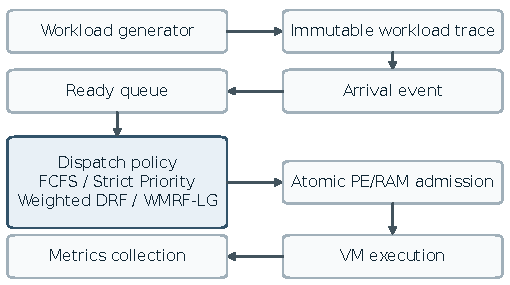
\includegraphics[width=.485\textwidth]{figures/system-architecture.pdf}
\hfill
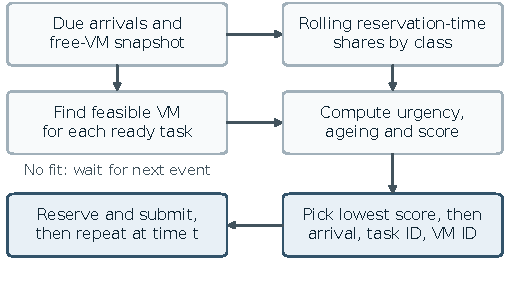
\includegraphics[width=.485\textwidth]{figures/algorithm-workflow.pdf}
\caption{Shared simulation lifecycle (left) and \wmrf{} dispatch decision (right). The broker refreshes capacity after each admission and reconsiders queued tasks after terminal release.}
\label{fig:architecture}
\end{figure*}

\subsection{Baseline scheduling policies}
\emph{FCFS} selects the feasible ready task with the earliest workload arrival, breaking ties by task identifier. \emph{Strict Priority} ranks Interactive above AI inference above Batch, applying FCFS and the same identifier tie-break within a class. It uses neither ageing nor fairness compensation. Both policies bypass an earlier or higher-priority task when it fits no VM. Each policy chooses the lowest-ID feasible VM.

\emph{\wdrf{}} is a project-specific heuristic that ranks classes by instantaneous weighted dominant share. For class $c$, it divides current reserved PEs and reserved RAM by total schedulable VM PEs and RAM, respectively, takes the larger of the two fractions, and divides by class entitlement $w_c$ from Table~\ref{tab:profiles}. The eligible class with the lowest share supplies the next task. Exact ties rank by ascending class identifier (\texttt{AI\_INFERENCE}, \texttt{BATCH}, \texttt{INTERACTIVE}), then by arrival and task identifier. It uses lowest-ID feasible placement, excludes urgency and ageing, and incorporates every new reservation in the next decision, even at the same timestamp. The heuristic borrows the dominant-share calculation from DRF \cite{ghodsi2011drf}. Its discrete reservations and VM-level placement carry no formal DRF guarantees.

\subsection{Proposed WMRF-LG policy}
\wmrf{} ranks tasks using rolling dominant-resource reservation-time accounting, latency urgency, and age. Let $t$ be elapsed simulated time since VM readiness, $W=60$ s the accounting window, and $L=\min(t,W)$. For reservation $k$, let $s_k$ be its dispatch time, $e_k$ its terminal release time (or $t$ if active), and $p_k$ and $m_k$ its PE count and RAM demand. Its accounted duration is
\begin{equation}
 d_k(t)=\max\{0,\min(t,e_k)-\max(t-L,s_k)\}.
 \label{eq:overlap}
\end{equation}
Released reservations ending at or before the window's left edge have zero overlap. With total schedulable VM capacities $P$ (PEs) and $M$ (RAM), the reservation-time shares and weighted dominant measure are
\begin{align}
 C(c,t)&=\frac{\sum_{k\in c}p_k d_k(t)}{P L},\notag\\
 R(c,t)&=\frac{\sum_{k\in c}m_k d_k(t)}{M L},\notag\\
 D(c,t)&=\frac{\max\{C(c,t),R(c,t)\}}{w_c}.
 \label{eq:service}
\end{align}
Both shares are zero for $L=0$. The denominator includes idle time. Simultaneous admissions add zero reservation time at the decision timestamp. The interval from dispatch through terminal release includes any delay before execution and the execution period. Only its overlap with the rolling window contributes to the score.

For workload arrival $a_j$, define $q_j(t)=\max(0,t-a_j)$. For an intrinsically feasible task with an SLA, urgency follows the implemented sum of normalized wait and normalized ideal service. The ageing threshold is $T_{\mathrm{age}}=60$ s:
\begin{align}
 U(j,t)&=
 \begin{cases}
 \min\{1,q_j(t)/\tau_j+b_j/\tau_j\},
   & \text{if SLA-feasible},\\
 0,& \text{otherwise},
 \end{cases}\label{eq:urgency}\\
 A(j,t)&=\min\{1,q_j(t)/T_{\mathrm{age}}\}.
 \label{eq:ageing}
\end{align}
The bounds are $0\leq U(j,t)\leq1$ and $0\leq A(j,t)\leq1$. Urgency reaches one at zero remaining ideal slack. Batch and intrinsically infeasible tasks have zero urgency. Ageing favors earlier admissions for older tasks of all classes but gives no formal starvation-freedom bound. The score is
\begin{equation}
 \operatorname{Score}(j,t)=D(c,t)-\lambda U(j,t)-\gamma A(j,t),
 \label{eq:score}
\end{equation}
where $c$ is the class of $j$, $\lambda=0.20$, and $\gamma=0.05$. The broker dispatches the feasible task with the lowest score. Exact Java \texttt{double} comparison resolves scores before comparing arrival time, task identifier and VM identifier. Entitlements influence order without creating per-class capacity caps. Eligible tasks can borrow available capacity, and the resulting reservations count in their class's rolling window.

\subsection{Pseudocode}
Figure~\ref{fig:pseudocode} combines the policy's read-only selection with the broker's admission loop. The current clock $t$ is shared by all iterations of a decision event. For $Q$ ready tasks, $V$ VMs, $R_a$ active reservations and $H$ released reservations retained in the window, one selection takes $O(QV+R_a+H)$ time. The broker repeats selection after each successful admission.

\begin{figure}[t]
\raggedright
\begin{algorithmic}[1]
\State Insert all due arrivals into ready queue at time $t$
\Loop
  \State Snapshot free PEs and RAM of each VM
  \State Compute $D(c,t)$ from \eqref{eq:overlap}--\eqref{eq:service}
  \State $\mathit{best}\gets\text{none}$
  \ForAll{ready tasks $j$ with $a_j\leq t$}
    \State $v\gets$ lowest-ID VM fitting both demands
    \If{such a VM exists}
      \State Compute $U(j,t)$ and $A(j,t)$ by \eqref{eq:urgency} and \eqref{eq:ageing}
      \State Compute $\operatorname{Score}(j,t)$ by \eqref{eq:score}
      \State Save the least tuple with its task and VM
      \Statex \hspace{\algorithmicindent} $(\operatorname{Score}(j,t),a_j,\operatorname{id}(j),\operatorname{id}(v))$
    \EndIf
  \EndFor
  \If{$\mathit{best}=\text{none}$}
    \State \Return
  \EndIf
  \State Remove the selected task from the ready queue
  \State Atomically reserve both resources and log start
  \State Bind and submit the Cloudlet to the selected VM
\EndLoop
\end{algorithmic}
\caption{WMRF-LG dispatch at an arrival or release event. The least tuple is stored in \textit{best}.}
\label{fig:pseudocode}
\end{figure}

\section{Results}
\subsection{Experimental configuration and measurements}
The evaluation used CloudSim Plus 8.5.7, JDK 25 and a Maven Java 17 compilation target. The three hosts each had four 1,000 MIPS PEs and 16,384 MB RAM. The six VMs each had two 1,000 MIPS PEs and 4,096 MB RAM. The four comparative policies and the four ablation variants each used all four workload scenarios, both configurations, and 20 deterministic seeds (42--61). The run manifest records 640 comparative and 640 ablation runs, for 1,280 runs and 153,600 successful task completions. No tasks failed, were cancelled, or were unfinished. The final verification report records 128 passing Maven tests.

One immutable trace was reused across all eight runs for a given scenario, configuration and seed. All 160 trace groups have a matching canonical SHA-256 fingerprint across runs. The versioned binary fingerprint includes the generation controls, class profiles and ordered task fields. Each run uses fresh simulator, Cloudlet, VM, broker and policy state. Full ablation reproduces the standard \wmrf{} run metrics and observation windows.

Response time equals successful completion minus workload arrival. Queue wait equals dispatch minus workload arrival. Both use completed tasks, and within-run response percentiles (P95 and P99) use nearest rank. Throughput divides completions by elapsed time from VM readiness to final successful completion. CPU and RAM reservation occupancy divides reserved PE-time and MB-time by total VM PE-time and MB-time over that full interval. The simulation does not measure physical CPU or RAM utilization. For class $c$, let $\bar C_c$ and $\bar R_c$ be the full-run occupancy fractions and $x_c=\max(\bar C_c,\bar R_c)/w_c$. The Jain index \cite{jain1984fairness} is
\begin{equation}
 J=\frac{(\sum_c x_c)^2}{n\sum_c x_c^2},
 \label{eq:jain}
\end{equation}
where $n$ counts arrived classes, including any with zero reserved capacity-time. The index is undefined when all $x_c$ are zero.

Each statistic is first computed per run and then averaged across seeds in its scenario, configuration and class. Paired differences are calculated per seed before averaging. The pointwise 95\% percentile bootstrap \cite{efron1986bootstrap} resamples 20 run statistics or 20 matched differences with replacement 10,000 times. The analysis uses the linear 2.5th and 97.5th percentiles of resampled means with NumPy's PCG64 generator seeded at 20261122. The intervals are exploratory and carry no multiplicity adjustment.

\subsection{Comparative performance}
Figures~\ref{fig:interactive} and \ref{fig:inference} summarize the mean response across seeds. Under Balanced original stress, mean Interactive response was 77.06 s for FCFS, 9.44 s for Strict Priority, 10.27 s for \wdrf{} and 9.78 s for \wmrf{}. In the same stratum, Strict Priority had Interactive P95/P99 of 17.49/20.94 s, versus 20.50/25.01 s for \wmrf{}. The WMRF-LG minus Strict Priority interval for mean Interactive response includes zero in that stratum (Table~\ref{tab:paired}). Strict Priority had the lowest mean Interactive response in all eight strata.

\begin{table}[t]
\caption{Selected matched differences in original stress}
\label{tab:paired}
\centering
\begin{tabular}{@{}llrr@{}}
\toprule
Scenario and metric & Baseline & $\Delta$ (s) & 95\% interval (s)\\
\midrule
Balanced, I response & FCFS & $-67.27$ & $[-80.48,-54.47]$\\
Balanced, I response & SP & $+0.34$ & $[-0.09,+0.83]$\\
Inf.-heavy, AI response & SP & $+70.33$ & $[+63.20,+77.52]$\\
Inf.-heavy, B max wait & SP & $-153.12$ & $[-172.45,-133.66]$\\
\bottomrule
\end{tabular}
\par\smallskip
{\footnotesize $\Delta$ is \wmrf{} minus baseline. I = Interactive, AI = AI inference, B = Batch, and SP = Strict Priority.}
\end{table}

Under Inference-heavy original stress, \wmrf{} had the highest mean inference response and the lowest mean per-run maximum Batch wait, at 210.29 s. Strict Priority had the lowest mean inference response and the highest mean per-run maximum Batch wait, at 363.41 s (Fig.~\ref{fig:batchwait}). The magnitude and direction of the paired differences in Table~\ref{tab:paired} show the cost of the observed Batch protection in that mix.

FCFS had the highest mean throughput in seven strata (Fig.~\ref{fig:throughput}). In Inference-heavy original stress, \wmrf{} led at 0.21895 tasks/s, compared with 0.21824 for \wdrf{}, 0.21752 for FCFS, and 0.21028 for Strict Priority. Jain values cluster closely within scenarios (Fig.~\ref{fig:fairness}). The four Inference-heavy stress means range from 0.695447 to 0.695453 despite the different latency and Batch wait outcomes. Table~\ref{tab:occupancy} compares full-run VM reservation occupancy in Balanced original stress over the 20 matched seeds.

\begin{table}[t]
\caption{Mean VM reservation occupancy in Balanced original stress}
\label{tab:occupancy}
\centering
\begin{tabular}{@{}lrr@{}}
\toprule
Policy & CPU (\%) & RAM (\%)\\
\midrule
FCFS & 90.34 & 49.34\\
Strict Priority & 89.46 & 48.86\\
\wdrf{} & 89.59 & 48.92\\
\wmrf{} & 89.15 & 48.69\\
\bottomrule
\end{tabular}
\end{table}

\begin{figure*}[t]
\centering
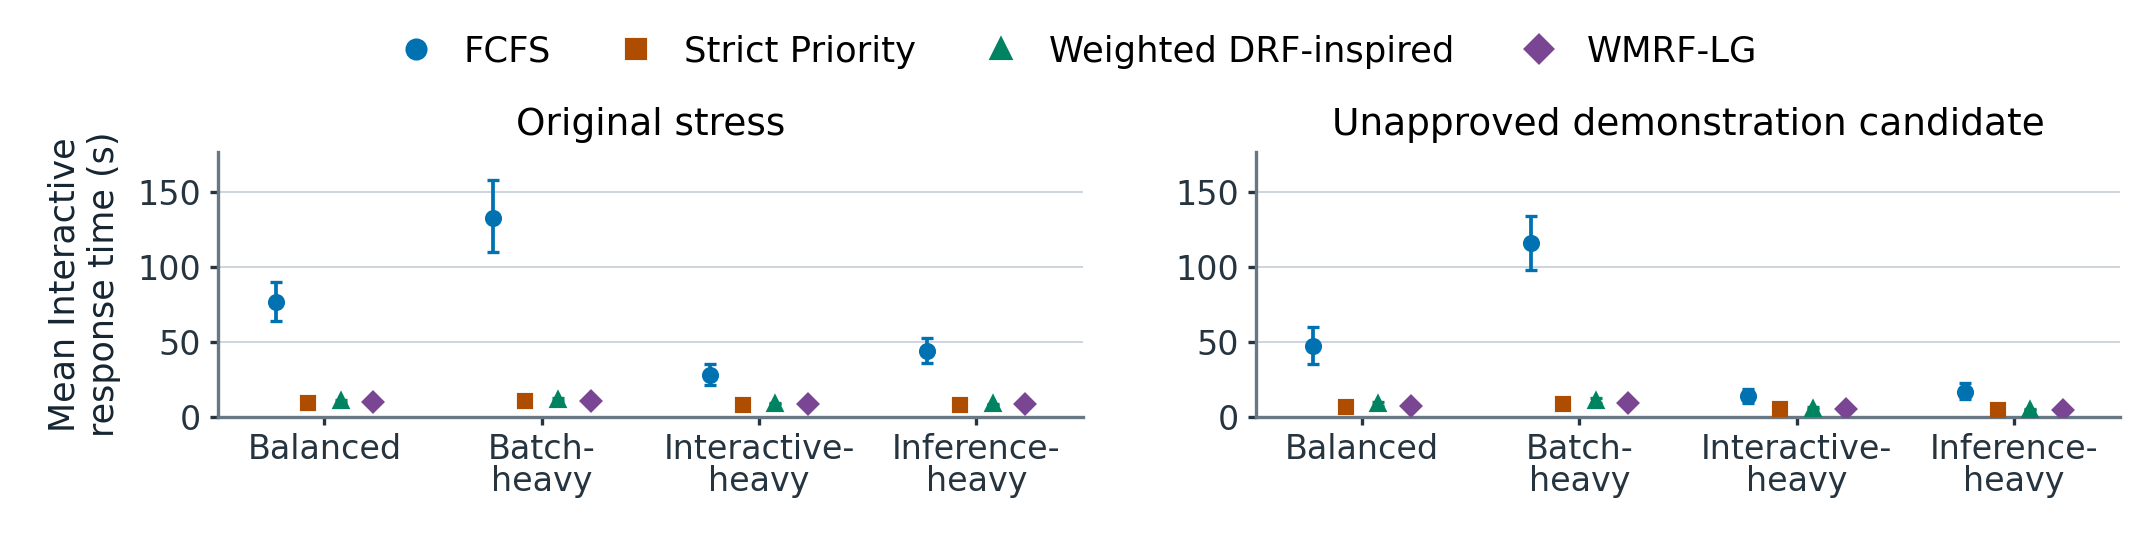
\includegraphics[width=\textwidth]{figures/interactive-latency.png}
\caption{Interactive response by policy. Across the results figures, points are means of run-level statistics and bars show pointwise 95\% bootstrap intervals across 20 seeds.}
\label{fig:interactive}
\end{figure*}

\begin{figure*}[t]
\centering
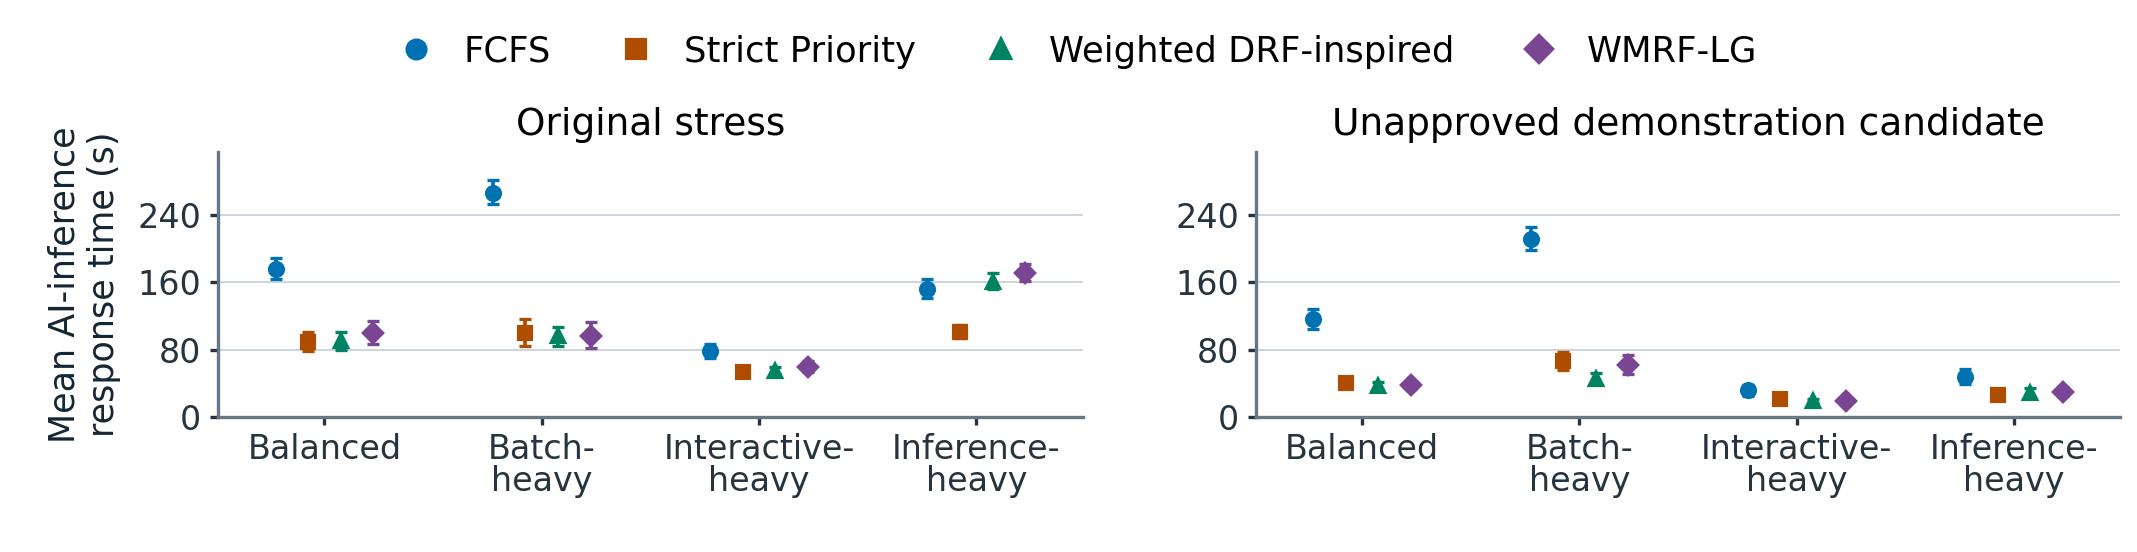
\includegraphics[width=\textwidth]{figures/inference-latency.png}
\caption{Mean AI-inference response by policy.}
\label{fig:inference}
\end{figure*}

\begin{figure*}[t]
\centering
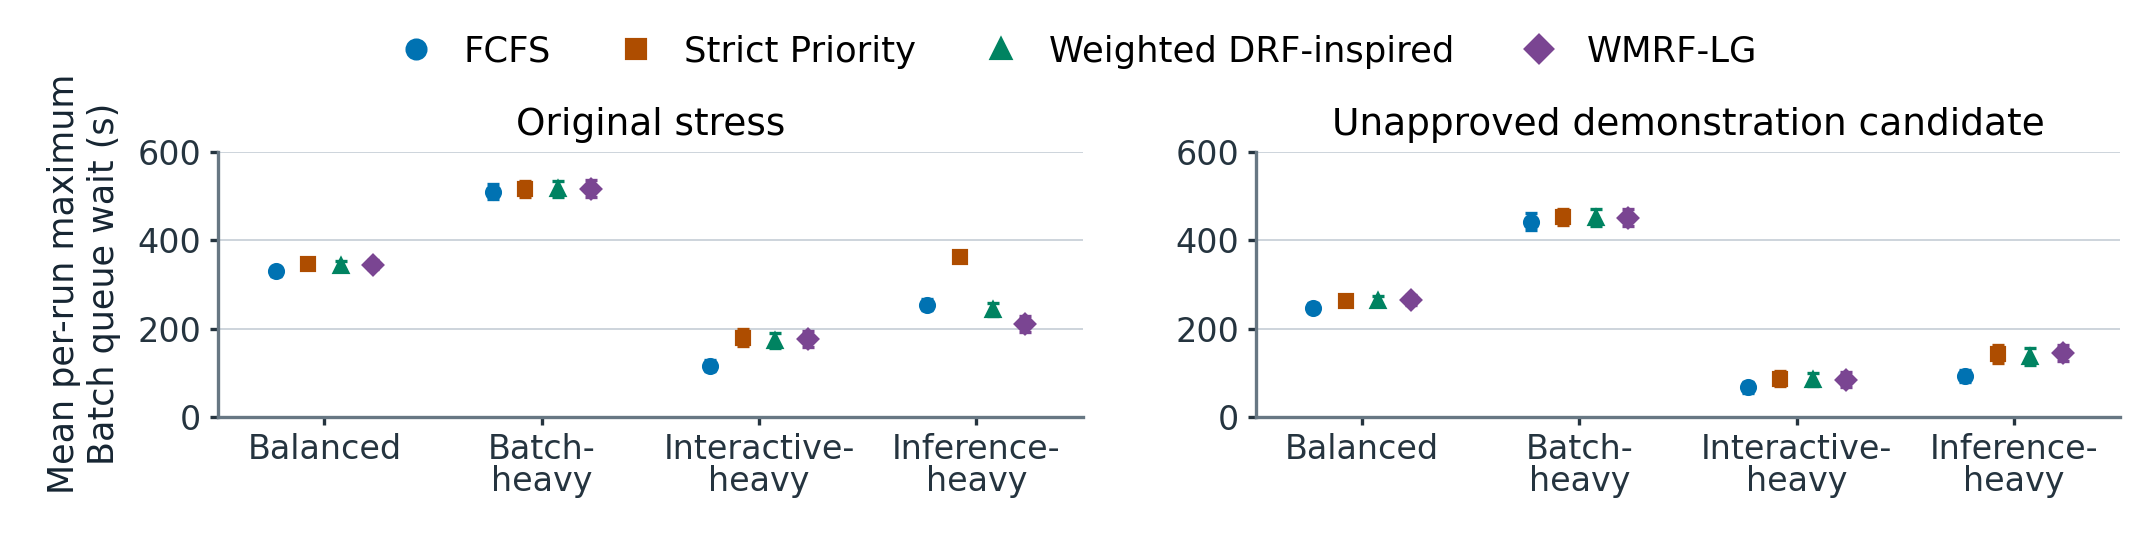
\includegraphics[width=\textwidth]{figures/batch-wait.png}
\caption{Mean of per-run maximum Batch queue waits. Queue wait ends at dispatch.}
\label{fig:batchwait}
\end{figure*}

\begin{figure*}[t]
\centering
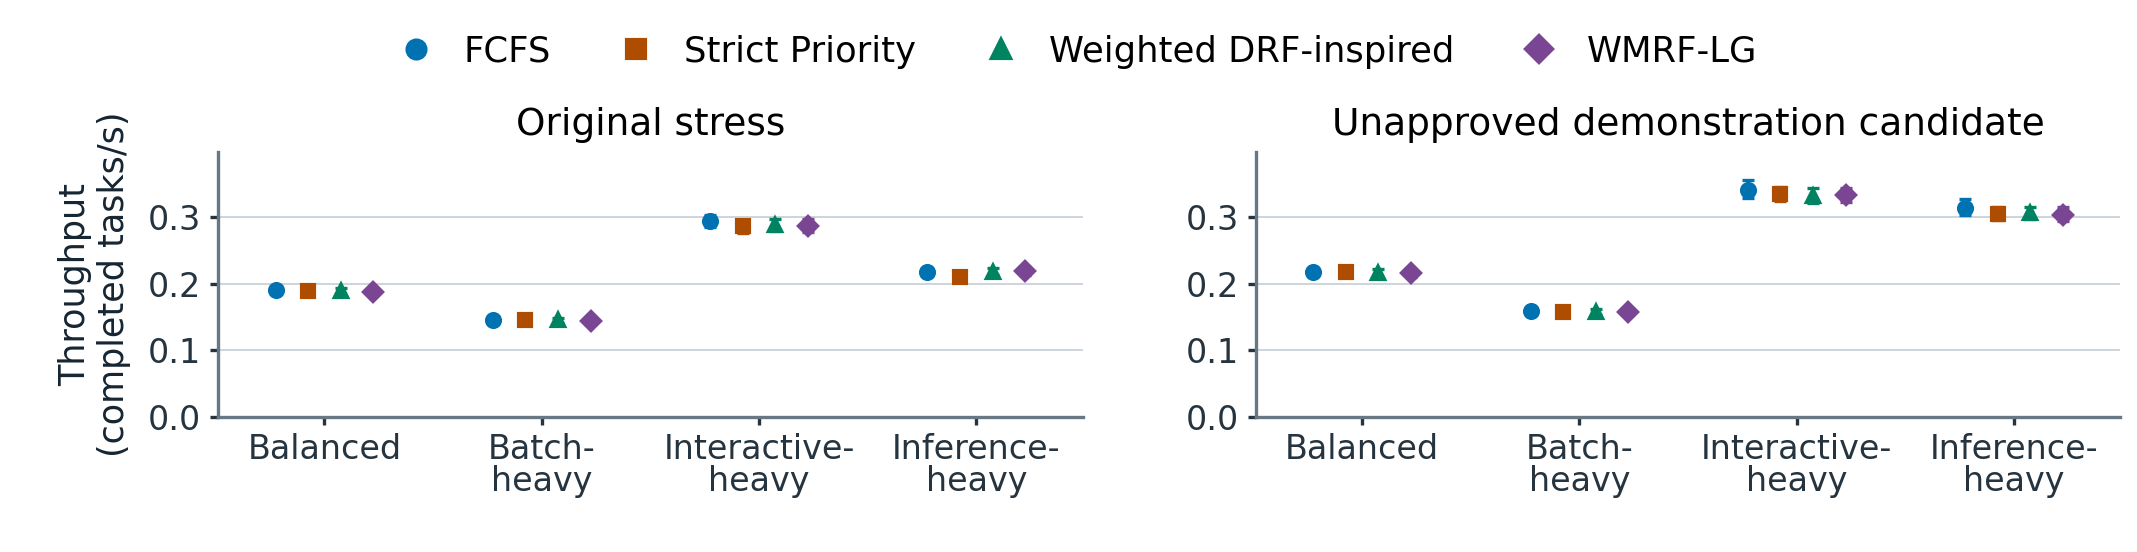
\includegraphics[width=\textwidth]{figures/throughput.png}
\caption{Aggregate throughput by policy over each run's observation interval.}
\label{fig:throughput}
\end{figure*}

\begin{figure*}[t]
\centering
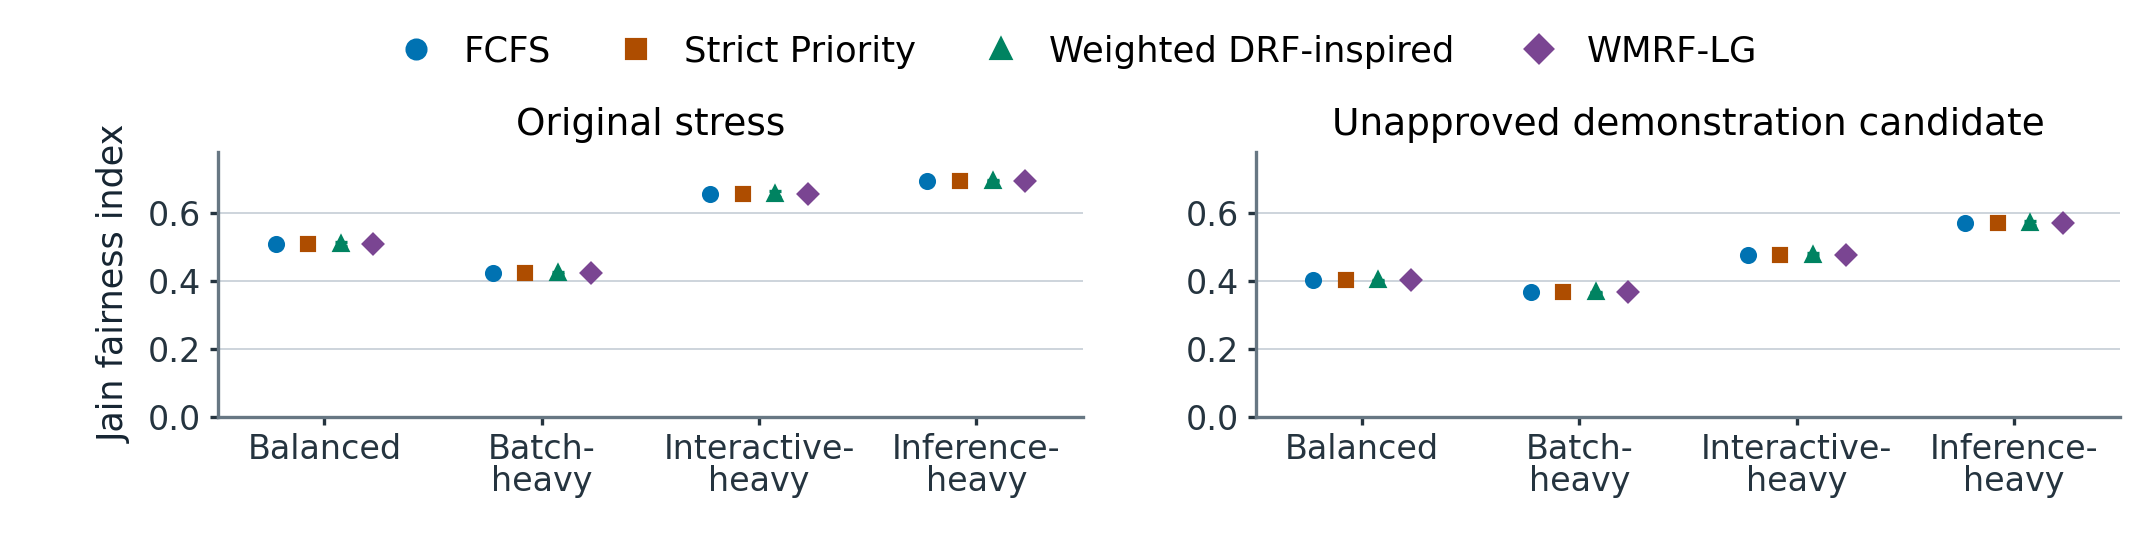
\includegraphics[width=\textwidth]{figures/fairness.png}
\caption{Jain fairness of entitlement-normalized dominant reservation-time shares, as defined in \eqref{eq:jain}.}
\label{fig:fairness}
\end{figure*}

\subsection{SLA and intrinsic feasibility}
A completed task misses its SLA if completion occurs after workload arrival plus the target. The overall miss ratio divides observed misses by all SLA-bearing tasks. The feasible-only ratio divides misses in the intrinsically feasible cohort by all intrinsically feasible tasks. Failed, cancelled, and unfinished SLA tasks would remain unresolved and are counted separately from observed misses. Batch has no SLA and is excluded from both denominators. A zero denominator leaves the ratio undefined.

Every original-stress inference task in the sampled traces was intrinsically infeasible, so its feasible-only miss ratio is undefined. Its ideal service bound already exceeded its deadline. In Balanced original stress, mean Interactive feasible-only miss rates were 84.5\% (FCFS), 54.8\% (Strict Priority), 61.9\% (\wdrf{}) and 47.6\% (\wmrf{}). Strict Priority's lower mean response and \wmrf{}'s lower feasible-only miss rate describe different metrics and task populations. In the Balanced demonstration candidate, all policies averaged a 99.2\% inference miss rate despite mean inference response ranging from 36.33 s to 115.89 s. The 10 s inference CPU bound equals the target in that candidate, so even a small delay can produce a miss.

\subsection{WMRF-LG ablation}
Table~\ref{tab:variants} lists the four variants. All retain the same weights, rolling window, eligibility rules and tie order. Differences are variant minus Full on each matched trace. The analysis also computes a within-seed interaction as Neither minus No latency minus No ageing plus Full. Figure~\ref{fig:ablation} shows absolute means for inference.

\begin{table}[t]
\caption{Ablation policies and coefficients}
\label{tab:variants}
\centering
\begin{tabular}{@{}lrr@{}}
\toprule
Policy identifier & $\lambda$ & $\gamma$\\
\midrule
\texttt{WMRF\_LG\_FULL} & 0.20 & 0.05\\
\texttt{WMRF\_LG\_NO\_LATENCY\_GUARD} & 0 & 0.05\\
\texttt{WMRF\_LG\_NO\_AGEING} & 0.20 & 0\\
\texttt{WMRF\_LG\_NO\_LATENCY\_NO\_AGEING} & 0 & 0\\
\bottomrule
\end{tabular}
\end{table}

Removing the latency guard increased mean inference response by 2.740 s in the Inference-heavy demonstration candidate (95\% paired interval $[0.904,5.131]$ s). Interactive effects were small and mixed. Removing ageing did not consistently increase Batch wait. For example, in the candidate the No ageing mean run-maximum Batch wait was 2.119 s higher in Batch-heavy and 0.530 s lower in Balanced than Full. Removing both terms changed the mean Jain index by at most $1.98\times10^{-5}$ across the eight strata.

\begin{figure*}[t]
\centering
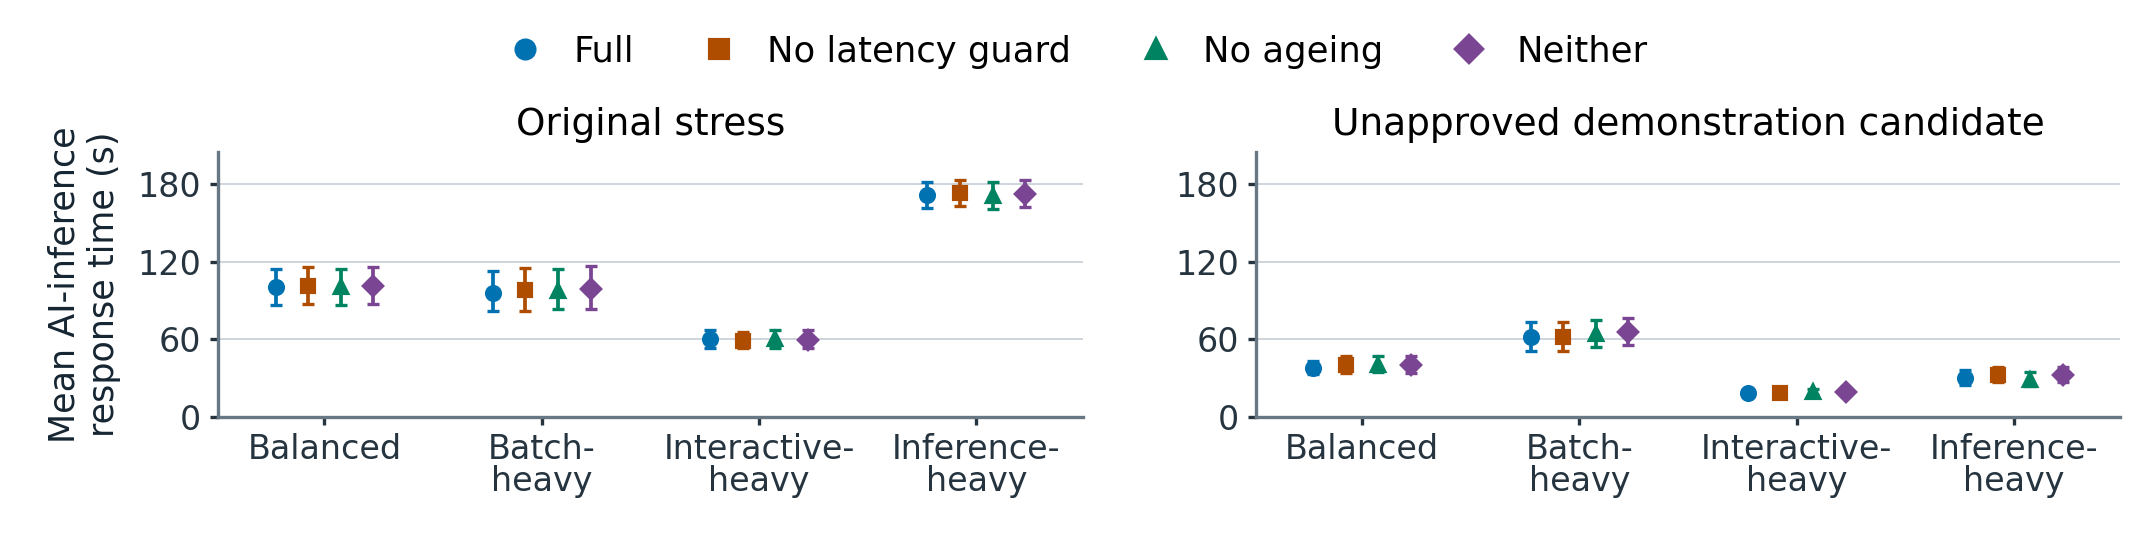
\includegraphics[width=\textwidth]{figures/ablation.png}
\caption{Mean AI-inference response for the four \wmrf{} ablation variants. Neither disables both urgency and ageing. Paired differences use the same traces and are reported in the text.}
\label{fig:ablation}
\end{figure*}

\section{Discussion}
All four policies are work-conserving subject to VM fit. Their differences arise from which feasible task is admitted next. Strict Priority consistently favors Interactive latency, and its fixed ordering can defer Batch when higher-priority tasks fit. Under Inference-heavy original stress, elevating inference relative to Batch protected inference latency at the cost of longer maximum Batch waits. All tasks eventually completed on these finite traces. The experiment measures deferral and cannot establish behavior under indefinite high-priority arrivals.

FCFS most often finished the fixed-size workload fastest, while older work delayed some later Interactive tasks. The \wdrf{} baseline reacts to instantaneous reserved-resource shares. \wmrf{} integrates reservations within a rolling window, including capacity borrowed when other classes lack feasible demand. The full-run Jain index captures similar class-level reservation-time totals across policies and can mask differences in dispatch order and waiting.

Urgency can affect inference directly in the demonstration candidate, where every inference task is intrinsically feasible. Under original stress, inference has zero urgency for the sampled traces, though a guard-driven change in Interactive ordering can affect inference indirectly. The ablation isolates these mechanisms only within the observed configurations. Ageing's bounded score contribution produced mixed Batch outcomes and establishes neither a general waiting-time improvement nor a starvation bound. The original stress and unapproved candidate also differ in service demand. Comparisons between them reflect both changed CPU lengths and changed feasibility, so they cannot isolate the effect of deadline slack.

The simulation uses one homogeneous VM topology, synthetic arrivals, and abstract inference tasks. Physical utilization, memory-bandwidth interference, and production co-location behavior are outside the instrumentation. The findings apply to the tested topology and workload traces. Pointwise bootstrap intervals characterize variation across seeds for individual metrics.

\section{Conclusion}
\wmrf{} combines rolling weighted dominant-resource reservation-time accounting, bounded urgency, ageing, and atomic CPU/RAM admission. Strict Priority led on mean Interactive response, and FCFS led on throughput in most strata. \wmrf{} shortened Batch waits at the expense of inference latency under Inference-heavy stress. Ablation found a latency-guard benefit in one inference stratum, mixed ageing effects, and negligible changes to full-run fairness. Future work should vary topology, burstiness, and deadline slack and measure class service and inference latency under real co-location.

\bibliographystyle{IEEEtran}
\bibliography{references}
\end{document}
